\documentclass[runningheads]{llncs}
\usepackage[T1]{fontenc}
\usepackage{graphicx}
\usepackage{hyperref}
\usepackage{color}
\usepackage{amsmath,amsfonts}
\usepackage{algorithm}
\usepackage{algpseudocode}
\usepackage{caption}
\usepackage{multirow}
\usepackage{tikz}
\usetikzlibrary{positioning}

% Custom commands
\newcommand{\pke}{\texttt{PKE}}
\newcommand{\keygen}{\texttt{Gen}}
\newcommand{\encrypt}{\texttt{Enc}}
\newcommand{\decrypt}{\texttt{Dec}}
\newcommand{\kem}{\texttt{KEM}}
\newcommand{\encap}{\texttt{Encap}}
\newcommand{\decap}{\texttt{Decap}}
\newcommand{\etm}{\texttt{EtM}}  % encrypt-then-mac
\newcommand{\mac}{\texttt{MAC}}
\newcommand{\sign}{\texttt{Sign}}
\newcommand{\verify}{\texttt{Verify}}
\newcommand{\pk}{\texttt{pk}}
\newcommand{\sk}{\texttt{sk}}
\newcommand{\pco}{\texttt{PCO}}
\newcommand{\cvo}{\texttt{CVO}}
\newcommand{\leftsample}{\stackrel{\$}{\leftarrow}}
\newcommand{\llbrack}{[\![}
\newcommand{\rrbrack}{]\!]}
\newcommand{\norm}[1]{\left\lvert #1 \right\rvert}
\newcommand{\adv}{\texttt{Adv}}
\newcommand{\fotplus}{\texttt{FOT+}}
\newcommand{\us}{\mu s}
\newcommand{\wt}{\mathop{wt}}
\def\mlkemplus{\text{ML-KEM}^+}

\begin{document}

\title{Faster generic CCA secure KEM transformation using encrypt-then-MAC}
%\titlerunning{Abbreviated paper title}

\author{
    Ganyu Xu\inst{1} \and
    Guang Gong\inst{1} \and
    Kalikinkar Mandal\inst{2}
}
% First names are abbreviated in the running head.
% If there are more than two authors, 'et al.' is used.
\authorrunning{G. Xu et al.}

\institute{
    University of Waterloo, Waterloo, Ontario, Canada
    \email{\{g66xu,ggong\}@uwaterloo.ca} \and
    University of New Brunswick, Canada \email{kmandal@unb.ca}
}

\maketitle              % typeset the header of the contribution
%
\begin{abstract}
    TODO: write abstract later
    \keywords{
    First keyword  \and Second keyword \and Another keyword.
}
\end{abstract}

\section{Introduction}\label{sec:introduction}
Key encapsulation mechanism (KEM) is a public-key cryptographic primitive that allows two parties to establish a shared secret over an insecure communication channel. The accepted security requirement of a KEM is \textit{Indistinguishability under adaptive chosen ciphertext attack (IND-CCA)}. Intuitively speaking, IND-CCA security implies that no efficient adversary (usually defined as probabilistic polynomial time Turing machine) can distinguish a pseudorandom shared secret from a uniformly random bit string of identical length even with access to a decapsulation oracle. Unfortunately, CCA security is difficult to achieve from scratch. Early attempts at constructing CCA secure public-key cryptosystems using only heuristics argument and without using formal proof, such as RSA encryption in PKCS \#1 \cite{rfc2313} and RSA signature ISO 9796 \cite{ISO9796-1}, were badly broken with sophisticated cryptanalysis \cite{DBLP:conf/crypto/Bleichenbacher98,coppersmith1999iso,DBLP:conf/crypto/CoronNS99}. Afterwards, provable chosen ciphertext security became a necessity for new cryptographic protocols. There have been many provable CCA secure constructions since then. Notable examples include Optimal Asymmetric Encryption Padding (OAEP) \cite{DBLP:conf/eurocrypt/BellareR94}, which is combined with RSA \cite{DBLP:conf/crypto/FujisakiOPS01} into the widely adopted RSA-OAEP. The Fujisaki-Okamoto transformation \cite{DBLP:conf/crypto/FujisakiO99,DBLP:conf/tcc/HofheinzHK17} is another generic CCA secure transformation that was thoroughly studied and widely adopted, particularly by many KEM candidates in NIST's Post Quantum Cryptography (PQC) standardization project.

Chosen ciphertext security is a solved problem within the context of symmetric cryptography. It is well understood that authenticated encryption can be achieved by combining a semantically secure symmetric encryption scheme with an existentially unforgeable message authentication code (MAC) using either the ``encrypt-then-MAC'' (AES-GCM, ChaCha20-Poly1305) or ``MAC-then-encrypt'' pattern (AES-CCM)\cite{DBLP:conf/asiacrypt/BellareN00,DBLP:conf/crypto/Krawczyk01}. However, adapting this technique for public-key cryptosystems is challenging, since the two communicating parties do not have a pre-shared symmetric key. The first attempt at such adaption is the Diffie-Hellman integrated encryption scheme (DHIES) \cite{DBLP:journals/iacr/AbdallaBR99,DBLP:conf/ctrsa/AbdallaBR01} proposed by Abdalla, Bellare, and Rogaway, who proved its chosen ciphertext security under a non-standard but well studied assumption called ``Gap Diffie-Hellman problem'' \cite{DBLP:conf/pkc/OkamotoP01}. DHIES and its variations appeared in international standards such as IEEE P1363a\cite{P1363a-2004} and ANSI X9.63\cite{ansi-x9.63}.

\subsection{Our contributions}\label{sec:our-contributions}
Our contributions are as follows:

\subsubsection{Generic CCA secure KEM transformation.} We propose the ``encrypt-then-MAC'' KEM transformation. Our transformation constructs a KEM with provable CCA security under the random oracle model using a public-key encryption scheme (PKE) with one-wayness under plaintext-checking attack and a message authentication code with existential unforgeability. Compared to the Fujisaki-Okamoto transformation, which is widely adopted by many KEM candidates in NIST's Post Quantum Cryptography (PQC) standardization project, our transformation replaces \textit{de-randomization} (which might degrade the security of a randomized cryptosystem) and \textit{re-encryption} (which is computationally inefficient and introduces additional risk of side channels) with computing MAC tag. We also provided concrete cryptanalysis on possible real-world attacks.

\subsubsection{Instantiation with ElGamal and McEliece cryptosystem.} We applied our KEM transformation to the ElGamal cryptosystem and the McEliece cryptosystems. We demonstrate that the ``encrypt-then-MAC'' KEM transformation is a generalization of DHIES by showing that the Gap Diffie-Hellman assumption is a special case of one-way security under plaintext checking attacks. We also surveyed plaintext checking attacks against many post quantum KEM candidates in the PQC standardizaton project.

\subsubsection{C implementation of McEliece+.} We implemented McEliece+ in C and benchmarked its performance. Compared to the reference implementation of Classic McEliece (which uses re-encryption), McEliece+ achieves significant decapsulation speedup at some minimal cost of encapsulation overhead, which results in 9-12\% increase in throughput (encapsulation + decapsulation time).

\subsection{Related works}\label{sec:related-works}
\subsubsection{OAEP}
\textit{Optimal Asymmetric Encryption Padding (OAEP)} \cite{DBLP:conf/eurocrypt/BellareR94}, proposed by Mihir Bellare and Phillip Rogaway in 1994, was one of the earliest provably secure CCA transformations. However, Victor Shoup identified a non-trivial gap in OAEP's security proof that cannot be filled under ROM\cite{DBLP:conf/crypto/Shoup01}, although Fujisaki et al. later proved that RSA-OAEP is secure under the RSA assumption \cite{DBLP:conf/crypto/FujisakiOPS01}. RSA-OAEP is widely used in secure communication protocols such as TLS 1.2. The main drawback of OAEP is that it requires its input to be an one-way trapdoor permutation, which is difficult to find. To this day, RSA remains the only viable candidate to apply OAEP to.

\subsubsection{REACT/GEM} Okamoto and Pointchval proposed REACT \cite{DBLP:conf/ctrsa/OkamotoP01} (Figure \ref{fig:react}) in 2001, followed by GEM \cite{DBLP:conf/ctrsa/CoronHJPPT02} in 2002. Both are generic CCA transformation with security proved under ROM. Okamoto and Pointcheval first defined the security notion of one-wayness under plaintext checking attack (OW-PCA) and reduced the CCA security of the transformation to the OW-PCA security of the input public-key cryptosystem.

\begin{figure}[H]
    \centering
    \begin{minipage}[t]{0.45\textwidth}
        \begin{algorithm}[H]
            \caption*{$\encrypt_\text{REACT}(\pk, m)$}
            \begin{algorithmic}[1]
                \State $w \leftarrow \mathcal{M}_\pke$
                \State $c_1 \leftarrow \encrypt(\pk, w)$
                \State $k \leftarrow G(w)$
                \State $c_2 \leftarrow \mathcal{E}_k(m)$
                \State $c_3 \leftarrow H(w, m, c_1, c_2)$
                \State \Return $(c_1, c_2, c_3)$
            \end{algorithmic}
        \end{algorithm}
    \end{minipage}\hfill
    \begin{minipage}[t]{0.45\textwidth}
        \begin{algorithm}[H]
            \caption*{$\decrypt_\text{REACT}(\sk, c)$}
            \begin{algorithmic}[1]
                \Require $(c_1, c_2, c_3) \leftarrow c$
                \State $\hat{w} \leftarrow \decrypt(\sk, c_1)$
                \State $\hat{k} \leftarrow G(\hat{w})$
                \State $\hat{m} \leftarrow \mathcal{D}_{\hat{k}}(c_2)$
                \If{$H(\hat{w}, \hat{m}, c_1, c_2) = c_3$}
                    \State \Return $\hat{m}$
                \Else
                    \State \Return $\bot$
                \EndIf
            \end{algorithmic}
        \end{algorithm}
    \end{minipage}
    \caption{Given PKE $(\keygen, \encrypt, \decrypt)$, SKE $(\mathcal{E}, \mathcal{D})$, and hash functions $G, H$, REACT constructs a hybrid PKE $(\keygen_\text{REACT}, \encrypt_\text{REACT}, \decrypt_\text{REACT})$}\label{fig:react}
\end{figure}

\begin{figure}[H]
    \centering
    \begin{minipage}[t]{0.45\textwidth}
        \begin{algorithm}[H]
            \caption*{$\encrypt_\text{GEM}(\pk, m)$}
            \begin{algorithmic}[1]
                \State $r \leftarrow \mathcal{R}$
                \State $s \leftarrow F(m, r)$
                \State $w \leftarrow s \Vert (r \oplus H(s))$
                \State $c_1 \leftarrow \encrypt(\pk, w)$
                \State $k \leftarrow G(w, c_1)$
                \State $c_2 \leftarrow \mathcal{E}_k(m)$
                \State \Return $(c_1, c_2)$
            \end{algorithmic}
        \end{algorithm}
    \end{minipage}
    \begin{minipage}[t]{0.45\textwidth}
        \begin{algorithm}[H]
            \caption*{$\decrypt_\text{GEM}(\sk, c)$}
            \begin{algorithmic}[1]
                \Require $(c_1, c_2) \leftarrow c$
                \State $\hat{w} \leftarrow \decrypt(\sk, c_1)$
                \State $(\hat{s}, \hat{t}) \leftarrow \hat{w}$
                \State $\hat{r} \leftarrow \hat{t}\oplus H(\hat{s})$
                \State $\hat{k} \leftarrow G(\hat{w}, c_1)$
                \State $\hat{m} \leftarrow \mathcal{D}_{\hat{k}}(c_2)$
                \If{$F(\hat{m}, \hat{r}) = \hat{s}$}
                    \State \Return $\hat{m}$
                \Else \State \Return $\bot$
                \EndIf
            \end{algorithmic}
        \end{algorithm}
    \end{minipage}
    \caption{Given PKE $(\keygen, \encrypt, \decrypt)$, SKE $(\mathcal{E}, \mathcal{D})$, and hash functions $F, G, H$, GEM constructs a hybrid PKE $(\keygen_\text{GEM}, \encrypt_\text{GEM}, \decrypt_\text{GEM})$}\label{fig:gem}
\end{figure}

\subsubsection{Fujisaki-Okamoto transformation}
Fujisaki and Okamoto proposed to construct CCA secure hybrid PKE by combining a OW-CPA secure PKE and a semantically secure symmetric-key encryption (SKE) scheme \cite{DBLP:conf/crypto/FujisakiO99}. The main techniques, namely \textit{de-randomization} and \textit{re-encrytion} were both introduced in the original proposal. Under ROM, Fujisaki and Okamoto reduced the CCA security of the hybrid PKE tightly to the semantic security of the input SKE and \textit{non-tightly} to the OW-CPA security of the input PKE (with loss factor $q$, the number of hash oracle queries). Later works extended the original proposal to build CCA secure KEM: KEM's security model makes building secure KEM simpler than building secure PKE, and it is well-known that combining a CCA secure KEM with a CCA secure data encapsulation mechanism (DEM), such as some authenticated encryption scheme (e.g. AES-GCM, AES-CCM, ChaCha20-Poly1305), results in a CCA secure hybrid PKE \cite{DBLP:journals/iacr/Shoup01,DBLP:conf/eurocrypt/Shoup00a}. Further studies \cite{DBLP:conf/ima/Dent03,DBLP:conf/tcc/HofheinzHK17,DBLP:journals/iacr/BernsteinP18,DBLP:conf/asiacrypt/HovelmannsHM22,DBLP:conf/pqcrypto/XagawaY19,DBLP:conf/crypto/JiangZCWM18} gave tighter security bounds, accounted for decryption failures in the underlying PKE, and analyzed the security under quantum random oracle model (QROM). To this day, the Fujisaki-Okamoto transformation is the only known generic CCA secure transformation that can convert OW-CPA/IND-CPA PKE into a CCA secure KEM. Because of the minimal input requirement and the simple construction, the Fujisaki-Okamoto transformation was widely adopted among post-quantum KEM candidates submitted to the PQC standardization project, including Kyber \cite{DBLP:conf/eurosp/BosDKLLSSSS18}, Saber \cite{DBLP:conf/africacrypt/DAnversKRV18}, FrodoKEM \cite{DBLP:conf/ccs/BosCDMNNRS16}, and Classic McEliece \cite{DBLP:conf/ches/BernsteinCS13}.

Despite its widespread adoption, the Fujisaki-Okamoto transformation has many flaws: \begin{itemize}
    \item \textbf{Computational inefficiency.} In all variants of Fujisaki-Okamoto transformation, decapsulation routine needs to re-encrypt the decryption to ensure ciphertext non-malleability. For input PKE whose encryption routine carries significant computational cost, such as most lattice-based cryptosystems, re-encryption substantially slows down decapsulation.
    \item \textbf{Side-channel vulnerability.} Re-encryption introduces side-channels that can leak information about the decrypted PKE plaintext. As demonstrated in \cite{DBLP:journals/tches/UenoXTITH22,DBLP:journals/tches/TanakaUXITH23,DBLP:conf/acns/Huguenin-Dumittan20}, these side-channels can be converted into efficient plaintext-checking attacks that can fully recover the secret key
    \item \textbf{Security degradation.} \textit{de-randomization} can degrade the security of a randomized PKE. Where the security parameters did not account for this loss, the security of the KEM can fall below the expected level. Consequently, larger parameters are necessary to account for the security loss, which slows down the cryptosystem \cite{cryptoeprint:2021/912,DBLP:journals/iacr/Bernstein21}.
\end{itemize}

\subsection{Paper organization}\label{sec:paper-organization}
In Section \ref{sec:preliminaries}, we review the preliminary definitions and theorems. In Section \ref{sec:the-enc-then-mac-transformation}, we present the encrypt-then-MAC KEM transformation, proves its CCA security, and discusses practical attacks. In Section \ref{sec:application-to-elgamal}, we show that the encrypt-then-MAC transformation is a generalization of DHIES by applying it to the ElGamal cryptosystem. In Section \ref{sec:application-to-mceliece}, we present McEliece+, an instantiation of the encrypt-then-MAC transformation, benchmark, and compare the performance of McEliece+ with Classic McEliece.

\section{Preliminaries}\label{sec:preliminaries}
\subsection{Public-key encryption scheme}
\subsubsection{Syntax} A public-key encryption scheme (PKE) is a collection fo three routines $(\keygen, \encrypt, \decrypt)$ defined over some plaintext space $\mathcal{M}$ and some ciphertext space $\mathcal{C}$. Key generation $(\pk, \sk) \leftarrow \keygen(1^\lambda)$ is a randomized routine that returns a keypair consisting of a public encryption key and a secret decryption key. The encryption routine $\encrypt: (\pk, m) \mapsto c$ encrypts the input plaintext $m$ under the input public key $\pk$ and produces a ciphertext $c$. The decryption routine $\decrypt: (\sk, c) \mapsto m$ decrypts the input ciphertext $c$ under the input secret key and produces the corresponding plaintext. Where the encryption routine is randomized, we denote the randomness by a coin $r \in \mathcal{R}$ where $\mathcal{R}$ is called the coin space. Decryption routines are assumed to always be deterministic.

\subsubsection{Correctness} A PKE is $\delta$-correct if

\begin{equation*}
    E\left[\max_{m\in\mathcal{M}}
        P\left[ \decrypt(\sk, c) \neq m \mid c \leftarrow \encrypt(\pk, m)\right]
    \right] \leq \delta
\end{equation*}

Where the expectation is taken with respect to the probability distribution of all possible keypairs. For many lattice-based cryptosystems, decryption failures could leak information about the secret key, although the probability of a decryption failure is low enough that classical adversaries cannot exploit decryption failure more than they can defeat the underlying lattice problems.

\subsubsection{Security} The security of PKE's is conventionally discussed using adversarial games played between a challenger and an adversary \cite{DBLP:conf/stoc/GoldwasserM82}. In the OW-ATK game (Figure \ref{fig:pke-ow-atk-game}), the challenger samples a random keypair and a random encryption. The adversary is given the public key, the random encryption (also called the challenge ciphertext), and access to ATK, then asked to decrypt the challenge ciphertext.

\begin{figure}[H]
    \centering
    \begin{minipage}[t]{0.45\textwidth}
    \begin{algorithm}[H]
        \caption*{OW-ATK game}
        \begin{algorithmic}[1]
            \State $(\pk, \sk) \leftarrow \keygen(1^\lambda)$
            \State $m^\ast \leftarrow \mathcal{M}$
            \State $c^\ast \leftarrow \encrypt(\pk, m)$
            \State $\hat{m} \leftarrow A^\text{ATK}(1^\lambda, \pk, c^\ast)$
            \State \Return $\llbrack \hat{m} = m^\ast \rrbrack$
        \end{algorithmic}
    \end{algorithm}
    \end{minipage}
    \caption{The one-wayness game: challenger samples a random keypair and a random encryption, and the adversary wins if it correctly produces the decryption}\label{fig:pke-ow-atk-game}
\end{figure}

The advantage of an adversary is its probability of producing the correct decryption: $\text{Adv}^\text{OW-ATK}_\pke(A) = P[\hat{m} = m^\ast]$. A PKE is said to be OW-ATK secure if no efficient adversary can win the OW-ATK game with non-negligible probability.

\begin{figure}[H]
    \centering
    \begin{minipage}[t]{0.5\textwidth}
        \begin{algorithm}[H]
            \caption*{IND-ATK game}
            \begin{algorithmic}[1]
                \State $(\pk, \sk) \leftarrow \keygen(1^\lambda)$
                \State $(m_0, m_1) \leftarrow A^\text{ATK}(1^\lambda, \pk)$
                \State $b \leftarrow \{0,1\}$
                \State $c^\ast \leftarrow \encrypt(\pk, m_b)$
                \State $\hat{b} \leftarrow A^\text{ATK}(1^\lambda, \pk, c^\ast)$
                \State \Return $\llbrack \hat{b} = b \rrbrack$
            \end{algorithmic}
        \end{algorithm}
    \end{minipage}
    \caption{IND-ATK game: adversary is asked to distinguish the encryption of one message from another}\label{fig:pke-ind-atk-game}
\end{figure}

In the IND-ATK game (Figure \ref{fig:pke-ind-atk-game}), the adversary chooses two distinct messages and receives the encryption of one of them, randomly selected by the challenger. The advantage of an adversary is its probability of correctly distinguishing the ciphertext of one message from the other beyond blind guess: $\text{Adv}^\text{IND-ATK}_\pke(A) = \vert P[\hat{b} = b] - \frac{1}{2}\vert$. A PKE is said to be IND-ATK secure if no efficient adversary can win the IND-ATK game with non-negligible advantage.

In public-key cryptography, all adversaries are assumed to have access to the public key ($\text{ATK} = \text{CPA}$). If the adversary has access to a decryption oracle $\mathcal{O}_\decrypt: c \mapsto \decrypt(\sk, c)$, it is said to mount chosen-ciphertext attack (ATK = CCA). If the adversary has access to a plaintext-checking oracle (PCO) $\mathcal{O}_\pco: (m, c) \mapsto \llbrack m = \decrypt(\sk, c)\rrbrack$, then it is said to mount plaintext-checking attack (ATK = PCA).

\begin{equation*}
    \text{ATK} = \begin{cases}
        \text{CPA} & \mathcal{O}_\text{ATK} = \cdot \\
        \text{PCA} & \mathcal{O}_\text{ATK} = \mathcal{O}_\pco \\
        \text{CCA} & \mathcal{O}_\text{ATK} = \mathcal{O}_\decrypt \\
    \end{cases}
\end{equation*}

\subsection{Key encapsulation mechanism (KEM)}\label{sec:key-encapsulation-mechanism}
\subsubsection{Syntax} A key encapsulation mechanism (KEM) is a collection of three routines $(\keygen, \encap, \decap)$ defined over some ciphertext space $\mathcal{C}$ and some key space $\mathcal{K}$. Key generation $\keygen: 1^\lambda \mapsto (\pk, \sk)$ is a randomized routine that returns a keypair. Encapsulation $\encap: \pk \mapsto (c, K)$ is a randomized routine that takes a public encapsulation key and returns a pair of ciphertext $c$ and shared secret $K$ (also commonly referred to as session key). Decapsulation $\decap: (\sk, c) \mapsto K$ is a deterministic routine that uses the secret key $\sk$ to recover the shared secret $K$ from the input ciphertext $c$. Where the KEM chooses to reject invalid ciphertext explicitly, the decapsulation routine can also output the rejection symbol $\bot$. We assume a KEM to be perfectly correct:

$$
P\left[
    \decap(\sk, c) = K \mid (\pk, \sk) \leftarrow \keygen(1^\lambda); (c, K) \leftarrow \encap(\pk)
\right] = 1
$$

\subsubsection{Security} Similar to PKE security, the security of KEM is discussed using adversarial games. In the IND-ATK game (Figure \ref{fig:kem-ind-atk-game}), the challenger generates a random keypair and encapsulates a random secret; the adversary is given the public key and the ciphertext, then asked to distinguish the shared secret from a random bit string.

\begin{figure}
    \centering
    \begin{minipage}[t]{0.5\textwidth}
        \begin{algorithm}[H]
            \caption*{KEM IND-ATK Game}
            \begin{algorithmic}[1]
                \State $(\pk, \sk) \leftarrow \keygen((1^\lambda))$
                \State $(c^\ast, K_0) \leftarrow \encap(\pk)$
                \State $K_1 \leftarrow \mathcal{K}$
                \State $b \leftarrow \{0,1\}$
                \State $\hat{b} \leftarrow A^\texttt{ATK}(1^\lambda, \pk, c^\ast, K_b)$
                \State \Return $\llbrack \hat{b} = b \rrbrack$
            \end{algorithmic}
        \end{algorithm}
    \end{minipage}
    \caption{The IND-ATK game for KEM}\label{fig:kem-ind-atk-game}
\end{figure}

The advantage of an adversary is its probability of winning beyong blind guess. A KEM is said to be IND-ATK secure if no efficient adversary can win the IND-ATK game with non-negligible advantage.

$$
\texttt{Adv}^\texttt{IND-ATK}(A) = \left\vert P\left[
    A^\texttt{ATK}(1^\lambda, c^\ast, K_b) = b
    \mid \begin{aligned}
    &(\pk, \sk) \leftarrow \keygen(1^\lambda); \\
    &(c^\ast, K_0) \leftarrow \encap(\pk); \\
    &K_1 \leftarrow \mathcal{K}; b \leftarrow \{0,1\}
    \end{aligned}
\right] - \frac{1}{2}
\right\vert
$$

By default, all adversaries are assumed to have the public key, with which they can mount chosen plaintext attacks (ATK = CPA). If the adversary as access to a decapsulation oracle $\mathcal{O}_\decap: c \mapsto \decap(\sk, c)$, it is said to mount a chosen-ciphertext attack (ATK = CCA).

\subsection{Message authentication code (MAC)}\label{sec:message-authentication-code}
\subsubsection{Syntax} A message authentication code (MAC) is a collection of two routines $(\sign, \verify)$ defined over some key space $\mathcal{K}$, some message space $\mathcal{M}$, and some tag space $\mathcal{T}$. The signing routine $\sign: (k, m) \mapsto t$ authenticates the message $m$ under the symmetric key $k$ by producing a tag $t$. The verification routine $\verify(k,m,t)$ outputs $1$ if the message-tag pair $(m, t)$ is authentic under the symmetric key $k$ and $0$ otherwise. Many MAC constructions are deterministic: for these constructions it is simpler to denote the signing routine by $t \leftarrow \mac(k, m)$, and verification done using a simple comparison. Some MAC constructions require a distinct or randomized nonce $r \leftarrow \mathcal{R}$, and the signing routine will take this additional argument $t \leftarrow \mac(k, m; r)$.

\subsubsection{Security} The standard security notion for a MAC is \textit{existential unforgeability under chosen message attack (EUF-CMA)}. We define it using an adversarial game in which an adversary has access to a signing oracle $\mathcal{O}_\sign: m \mapsto \sign(k, m)$ and tries to produce a valid message-tag pair that has not been queried from the signing oracle (Figure \ref{fig:euf-cma-game}).

\begin{figure}[H]
    \centering
    \begin{minipage}[t]{0.6\textwidth}
    \begin{algorithm}[H]
        \caption*{MAC EUF-CMA game}
        \begin{algorithmic}[1]
            \State $k^\ast \leftarrow \mathcal{K}$
            \State $(\hat{m}, \hat{t}) \leftarrow A^\texttt{CMA}()$
            \State \Return $\llbrack \verify(k^\ast, \hat{m}, \hat{t}) \land (\hat{m}, \hat{t}) \not\in \mathcal{O}_\sign \rrbrack$
        \end{algorithmic}
    \end{algorithm}
    \end{minipage}
    \caption{The signing oracle signs the queried message with the secret key. The adversary must produce a message-tag pair that has never been queried before}\label{fig:euf-cma-game}
\end{figure}

The advantage of the adversary is the probability that it successfully produces a valid message-tag pair. A MAC is said to be EUF-CMA secure if no efficient adversary has non-negligible advantage. Some MACs are \textit{one-time existentially unforgeable} (we call them one-time MAC), meaning that each secret key can be used to authenticate exactly one message. The corresponding security game is identical to the EUF-CMA game except for that the signing oracle will only answer up to one query.

\section{The encrypt-then-MAC transformation}\label{sec:the-enc-then-mac-transformation}
In this section we present the encrypt-then-MAC KEM transformation. The transformation constructs an IND-CCA secure KEM using an OW-PCA secure PKE and an existentially unforgeable MAC. Our scheme is inspired by DHIES, but differs from it in two key aspects: whereas DHIES reduces its CCA security specifically to the Gap Diffie-Hellman assumption \cite{DBLP:conf/pkc/OkamotoP01}, our construction's CCA security reduces generically to the PCA security of the the input PKE; in addition, we argue that if the PKE's plaintext space is large and the sampling method has sufficient entropy, then the MAC only needs to be one-time existentially unforgeable (Abdalla, Rogaway, and Bellare originally proposed to use HMAC and CBC-MAC, which are many-time secure MAC but less efficient than one-time MAC). The data flow of the encapsulation is illustrated in Figure \ref{fig:etm-encap-data-flow}

\begin{figure}[h]
    \centering
    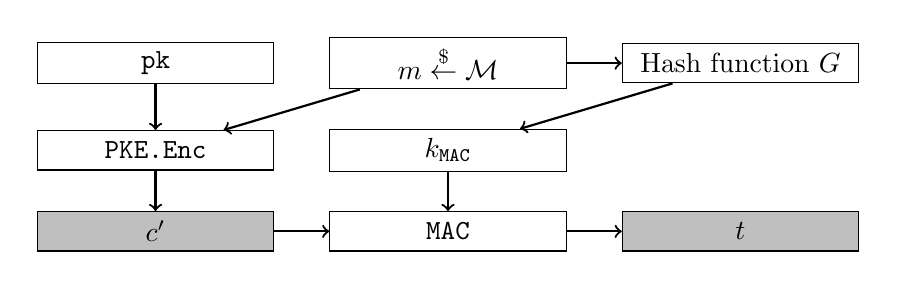
\begin{tikzpicture}
        \tikzstyle{rect} = [draw, rectangle, minimum width=3cm, minimum height=0.5cm]
        \tikzstyle{filledrect} = [draw, rectangle, minimum width=3cm, minimum height=0.5cm, fill=lightgray]
        \matrix [column sep=7mm, row sep=5mm] {
            \node (pk) [rect] {$\pk$}; &
            \node (m) [rect] {$m \leftsample \mathcal{M}$}; &
            \node (hashg) [rect] {Hash function $G$}; \\
            \node (pkeenc) [rect] {$\texttt{PKE.Enc}$}; &
            \node (mackey) [rect] {$k_\mac$}; \\
            \node (ct) [filledrect] {$c^\prime$}; &
            \node (mac) [rect] {$\mac$}; &
            \node (tag) [filledrect] {$t$}; \\
        };
        \draw[->, thick] (pk) -- (pkeenc);
        \draw[->, thick] (m) -- (pkeenc);
        \draw[->, thick] (m) -- (hashg);
        \draw[->, thick] (hashg) -- (mackey);
        \draw[->, thick] (pkeenc) -- (ct);
        \draw[->, thick] (mackey) -- (mac);
        \draw[->, thick] (ct) -- (mac);
        \draw[->, thick] (mac) -- (tag);
    \end{tikzpicture}

    \caption{Combining PKE with MAC using encrypt-then-MAC to ensure ciphertext integrity}\label{fig:etm-encap-data-flow}
\end{figure}


\section{Application to ElGamal}\label{sec:application-to-elgamal}
\section{McEliece+: applying encrypt-then-MAC to the McEliece cryptosystem}\label{sec:application-to-mceliece}

\bibliographystyle{splncs04}
\bibliography{biblio.bib}
\end{document}
